\subsection{Lab24: Constelación y FFT, Modulación BPSK}

%*********************
\begin{frame}{}

\pgfdeclareimage[width=\paperwidth,height=\paperheight]{bg}{imagenes/fondo_lab}
\setbeamertemplate{background}{\pgfuseimage{bg}}

\bfseries{\textrm{\LARGE Lab24\\ \Large Constelación y FFT \\Modulación BPSK}}
\raggedright
\end{frame}
%*********************

\begin{frame}
\pgfdeclareimage[width=\paperwidth,height=\paperheight]{bg}{imagenes/fondo3}
\setbeamertemplate{background}{\pgfuseimage{bg}}
   
  \frametitle{\underline{\textbf{Modulación BPSK}}}
  
   \begin{flushleft}
    La modulación BPSK o Modulación por desplazamiento de fase binaria, es una modulación  digital que se representa mediante un diagrama de constelación conformado por dos puntos equidistantes del origen de coordenadas.
   \end{flushleft}
   \begin{flushleft}
   Representa la modulación por desplazamiento de dos símbolos, con un bit de información cada uno, cada una de estas fases separadas a 180º, estos símbolos tienen un valor de salto de fase de 0º para (1) y de 180º para (0).
   \end{flushleft}
   \begin{flushleft}
   Este tipo de modulación digital (BPSK), es equivalente a la modulación 2-QAM, y  constelación de esta modulación se representa en el diagrama del plano I-Q.
   \end{flushleft} 
 \end{frame}
%*********************

\begin{frame}
\pgfdeclareimage[width=\paperwidth,height=\paperheight]{bg}{imagenes/fondo3}
\setbeamertemplate{background}{\pgfuseimage{bg}}
   
  \frametitle{\underline{\textbf{Modulación BPSK}}}
   \begin{flushleft}
   Como obtener la constelación en el plano de diagrama I-Q de una modulación BPSK, y su FFT.
   \end{flushleft}
   \begin{figure}[H]
\vspace{-3mm}
\centering
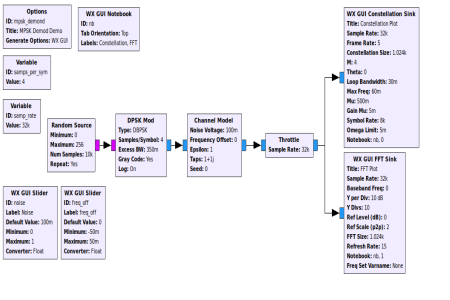
\includegraphics[width=0.9\textwidth]{Modulaciones_digitales/lab24/pdf/Psk_Diagrama.pdf}
\end{figure}
\end{frame}
%*********************

\begin{frame}
\pgfdeclareimage[width=\paperwidth,height=\paperheight]{bg}{imagenes/fondo3}
\setbeamertemplate{background}{\pgfuseimage{bg}}
   
  \frametitle{\underline{\textbf{Constelación y FFT; BPSK}}}
   \begin{flushleft}
 Para observar la constelación y la señal FFT de una modulación BPSK, se tiene en cuenta la utilización del Channel Model y Random Source.
   \end{flushleft}
   \begin{figure}[H]
   \centering
   \vspace{-3mm}
  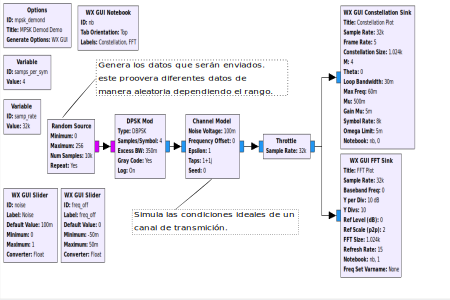
\includegraphics[width=0.9\textwidth]{Modulaciones_digitales/lab24/pdf/PskRamdonsourceChannel.pdf} 
   \end{figure}
\end{frame}
%*********************   

 \begin{frame}
 \pgfdeclareimage[width=\paperwidth,height=\paperheight]{bg}{imagenes/fondo3}
\setbeamertemplate{background}{\pgfuseimage{bg}}
   
  \frametitle{\underline{\textbf{Configuración de Bloque}}}
   \begin{flushleft}
   Para generar los datos que serán enviados mediante el canal de transmición, se debe configurar el bloque Random Source. 
   \end{flushleft}
   \begin{figure}[H]
   \centering
   \vspace{-3mm}
  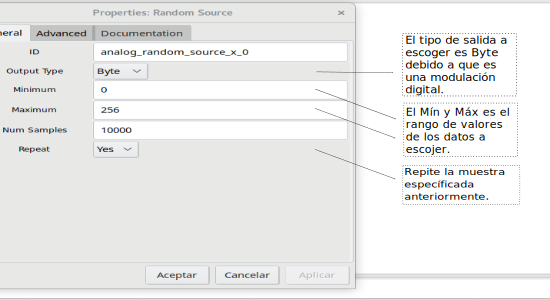
\includegraphics[width=0.9\textwidth]{Modulaciones_digitales/lab24/pdf/PskRamdonsource_configuracion.pdf} 
   \end{figure}
 \end{frame}
%********************* 

 \begin{frame}
  \pgfdeclareimage[width=\paperwidth,height=\paperheight]{bg}{imagenes/fondo3}
\setbeamertemplate{background}{\pgfuseimage{bg}}
   
  \frametitle{\underline{\textbf{Configuración de Modulador}}}
 
   \begin{flushleft}
  Realizamos la configuración previa en el bloque para realizar la modulación BPSK
   \end{flushleft}
   \begin{figure}[H]
   \centering
   \vspace{-3mm}
   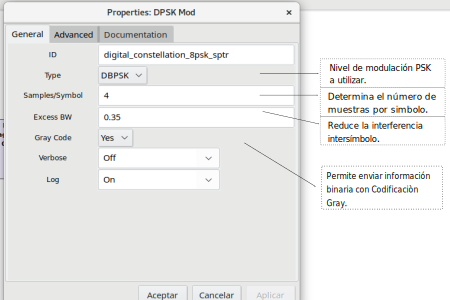
\includegraphics[width=0.9\textwidth]{Modulaciones_digitales/lab24/pdf/PskModulador_configuracion.pdf} 
   \end{figure}
   \begin{flushleft}
  En la modulación BPSK, la información que se transmite a través de un canal de    comunicación se envía durante la fase de la portadora, una fase partícular de 180º se usa para representar la información discreta.
  \end{flushleft}  
 \end{frame}
%********************* 

 \begin{frame}
 \pgfdeclareimage[width=\paperwidth,height=\paperheight]{bg}{imagenes/fondo3}
\setbeamertemplate{background}{\pgfuseimage{bg}}
   
  \frametitle{\underline{\textbf{Configuración del Canal}}}
 
   \begin{flushleft}
    La simulación del canal se hace mediante el bloque Channel Model, este simula un canal AWGN.
   \end{flushleft}
   \begin{figure}[H]
   \centering
   \vspace{-3mm}
   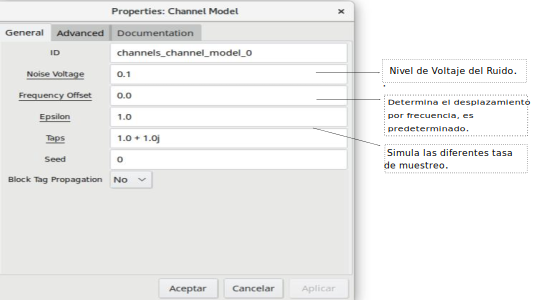
\includegraphics[width=0.9\textwidth]{Modulaciones_digitales/lab24/pdf/Pskchannel_configuracion.pdf} 
   \end{figure} 
 \end{frame} 
%*********************  

 \begin{frame}
 \pgfdeclareimage[width=\paperwidth,height=\paperheight]{bg}{imagenes/fondo3}
\setbeamertemplate{background}{\pgfuseimage{bg}}
   
  \frametitle{\underline{\textbf{Constelación BPSK}}}
   \begin{flushleft}
   En la modulación se observa el desfase de 180º entre cada símbolo de la constelación del diagrama I-Q, donde I representa la fase y Q la cuadratura, pero en este caso la cuadratura no es utilizada ya que no es una modulación de tipo cuadrifásica.
   \end{flushleft}
   \begin{figure}[H]
   \centering
   \vspace{-3mm}
   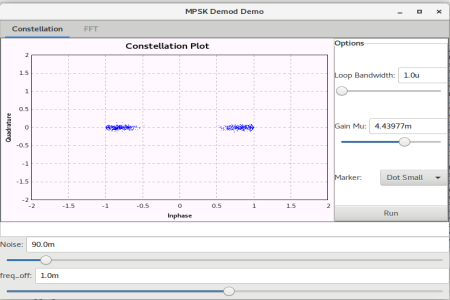
\includegraphics[width=0.8\textwidth]{Modulaciones_digitales/lab24/pdf/PskConstelacion.pdf}
   \end{figure}
 \end{frame}
%*********************

 \begin{frame}
 \pgfdeclareimage[width=\paperwidth,height=\paperheight]{bg}{imagenes/fondo3}
\setbeamertemplate{background}{\pgfuseimage{bg}}
   
  \frametitle{\underline{\textbf{Constelación BPSK}}}
 
    \begin{flushleft}
    Cuando exíste dispersión en los símbolos durante diferentes fases, se considera como un     error, debido que a que los símbolos que contienen información se perderán, es decir la información no será transmitida.
    \end{flushleft}
    \begin{figure}[H]
    \centering
    \vspace{-3mm}
    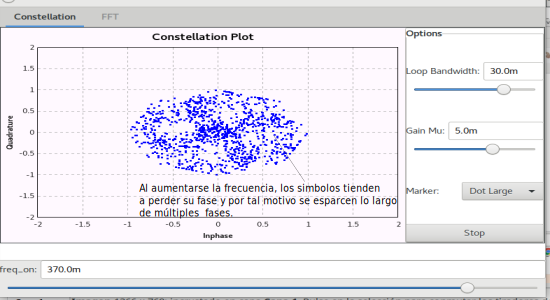
\includegraphics[width=0.9\textwidth]{Modulaciones_digitales/lab24/pdf/PskDispersiondesimbolos.pdf}
    \end{figure}
 \end{frame}
%*********************

\begin{frame}
\pgfdeclareimage[width=\paperwidth,height=\paperheight]{bg}{imagenes/fondo3}
\setbeamertemplate{background}{\pgfuseimage{bg}}
   
  \frametitle{\underline{\textbf{FFT, Modulación BPSK}}}
   \begin{flushleft}
  La FFT en la modulación BPSK, nos permite analizar y transformar una señal en el dominio de la frecuencia.
   \end{flushleft}
   \begin{figure}[H]
    \centering
    \vspace{-3mm}
   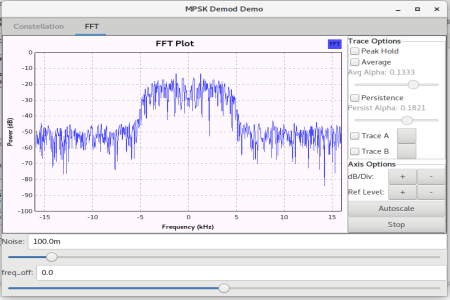
\includegraphics[width=0.9\textwidth]{Modulaciones_digitales/lab24/pdf/PskFFT.pdf}  
   \end{figure}
 \end{frame}
%*********************

\begin{frame}
\begin{figure}[H]
\centering
\vspace{-3mm}
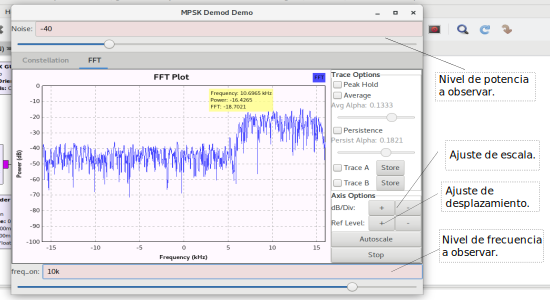
\includegraphics[width=0.9\textwidth]{Modulaciones_digitales/lab24/pdf/PskFFT_Ejemplo.pdf}   
\end{figure}
\end{frame}
  
